\documentclass[a4paper]{article}
\usepackage{vntex}
%\usepackage[english,vietnam]{babel}
%\usepackage[utf8]{inputenc}

%\usepackage[utf8]{inputenc}
%\usepackage[francais]{babel}
\usepackage{a4wide,amssymb,epsfig,latexsym,multicol,array,hhline,fancyhdr}
\usepackage{booktabs}
\usepackage{amsmath}
\usepackage{lastpage}
\usepackage[lined,boxed,commentsnumbered]{algorithm2e}
\usepackage{enumerate}
\usepackage{color}
\usepackage{graphicx}							% Standard graphics package
\usepackage{array}
\usepackage{tabularx, caption}
\usepackage{multirow}
\usepackage[framemethod=tikz]{mdframed}% For highlighting paragraph backgrounds
\usepackage{multicol}
\usepackage{rotating}
\usepackage{graphics}
\usepackage{geometry}
\usepackage{setspace}
\usepackage{epsfig}
\usepackage{tikz}
\usepackage{listings}
\usetikzlibrary{arrows,snakes,backgrounds}
\usepackage{hyperref}
\hypersetup{urlcolor=blue,linkcolor=black,citecolor=black,colorlinks=true} 
%\usepackage{pstcol} 								% PSTricks with the standard color package

\newtheorem{theorem}{{\bf Định lý}}
\newtheorem{property}{{\bf Tính chất}}
\newtheorem{proposition}{{\bf Mệnh đề}}
\newtheorem{corollary}[proposition]{{\bf Hệ quả}}
\newtheorem{lemma}[proposition]{{\bf Bổ đề}}

\everymath{\color{blue}}
%\usepackage{fancyhdr}
\setlength{\headheight}{40pt}
\pagestyle{fancy}
\fancyhead{} % clear all header fields
\fancyhead[L]{
 \begin{tabular}{rl}
    \begin{picture}(25,15)(0,0)
    \put(0,-8){
\includegraphics[width=8mm, height=8mm]{logoITSGUsmall.png}}
    %\put(0,-8){\epsfig{width=10mm,figure=hcmut.eps}}
   \end{picture}&
	%\includegraphics[width=8mm, height=8mm]{hcmut.png} & %
	\begin{tabular}{l}
		\textbf{\bf \ttfamily Trường Đại học Sài Gòn}\\
		\textbf{\bf \ttfamily Khoa Công Nghệ Thông Tin}
	\end{tabular} 	
 \end{tabular}
}
\fancyhead[R]{
	\begin{tabular}{l}
		\tiny \bf \\
		\tiny \bf 
	\end{tabular}  }
\fancyfoot{} % clear all footer fields
\fancyfoot[L]{\scriptsize \ttfamily Bài tập lớn môn Phát triển phần mềm mã nguồn mở - Niên khóa 2023-2024}
\fancyfoot[R]{\scriptsize \ttfamily Trang {\thepage}/\pageref{LastPage}}
\renewcommand{\headrulewidth}{0.3pt}
\renewcommand{\footrulewidth}{0.3pt}


%%%
\setcounter{secnumdepth}{4}
\setcounter{tocdepth}{3}
\makeatletter
\newcounter {subsubsubsection}[subsubsection]
\renewcommand\thesubsubsubsection{\thesubsubsection .\@alph\c@subsubsubsection}
\newcommand\subsubsubsection{\@startsection{subsubsubsection}{4}{\z@}%
                                     {-3.25ex\@plus -1ex \@minus -.2ex}%
                                     {1.5ex \@plus .2ex}%
                                     {\normalfont\normalsize\bfseries}}
\newcommand*\l@subsubsubsection{\@dottedtocline{3}{10.0em}{4.1em}}
\newcommand*{\subsubsubsectionmark}[1]{}
\makeatother

\definecolor{dkgreen}{rgb}{0,0.6,0}
\definecolor{gray}{rgb}{0.5,0.5,0.5}
\definecolor{mauve}{rgb}{0.58,0,0.82}

\lstset{frame=tb,
	language=Matlab,
	aboveskip=3mm,
	belowskip=3mm,
	showstringspaces=false,
	columns=flexible,
	basicstyle={\small\ttfamily},
	numbers=none,
	numberstyle=\tiny\color{gray},
	keywordstyle=\color{blue},
	commentstyle=\color{dkgreen},
	stringstyle=\color{mauve},
	breaklines=true,
	breakatwhitespace=true,
	tabsize=3,
	numbers=left,
	stepnumber=1,
	numbersep=1pt,    
	firstnumber=1,
	numberfirstline=true
}

\begin{document}

\begin{titlepage}
\begin{center}
TRƯỜNG ĐẠI HỌC SÀI GÒN \\
KHOA CÔNG NGHỆ THÔNG TIN
\end{center}
\vspace{1cm}

\begin{figure}[h!]
\begin{center}

\includegraphics[width=5cm]{logoITSGU.png}
\end{center}
\end{figure}

\vspace{1cm}

\begin{center}
\begin{tabular}{c} 
	\multicolumn{1}{l}{\textbf{{\Large PHÁT TRIỂN PHẦN MỀM MÃ NGUỒN MỞ}}}\\ 
	~~\\ 
	
	\\ 
	\multicolumn{1}{l}{\textbf{{\Large Xây dựng ứng dụng game}}}\\ 
	\\ 
	
	\textbf{{\Large Kéo, búa, bao nhiều người chơi trên PYTHON}}\\
\\ 
	{\Large Nhóm 15}\\ 
	
\end{tabular}
\end{center}

\vspace{1cm}

\begin{table}[h]
\centering
\begin{tabular}{rll}
& GVHD: &Từ Lãng Phiêu\\
& Thành viên nhóm:& Lê Quỳnh Thiên Hương - 3120560036\\
& & Bùi Thị Yến Nhi - 3120560069\\
& & Nhâm Gia Phát - 3120560071\\
&Email liên hệ:&thienhuong6935@gmail.com
% & & SV3 - MSSV \\
% & & SV4 - MSSV\\
\end{tabular}
\vspace{1.5 cm}
\end{table}

\begin{center}

{\footnotesize TP. HỒ CHÍ MINH, THÁNG 2/2024}
\end{center}
\end{titlepage}


\thispagestyle{empty}

\newpage
\tableofcontents
\newpage

%%%%%%%%%%%%%%%%%%%%%%%%%%%%%%%%%


%%%%%%%%%%%%%%%%%%%%%%%%%%%%%%%%%
\section{PHẦN GIỚI THIỆU}
Dự án này hướng đến việc xây dựng một ứng dụng game Kéo, Búa, Bao nhiều người chơi bằng Python. Game sẽ bao gồm hai người chơi trực tuyến đối đầu với nhau theo quy tắc truyền thống của trò chơi Kéo, Búa, Bao. Sử dụng thư viện Pygame để tạo giao diện người dùng và một máy chủ mạng để quản lý kết nối và tương tác giữa các người chơi.
Việc hoàn thành dự án này sẽ cung cấp một cái nhìn sâu sắc về cách xây dựng một ứng dụng trò chơi từ đầu đến cuối, bao gồm thiết kế giao diện người dùng, lập trình logic trò chơi, và quản lý kết nối mạng.



\newpage
%%%%%%%%%%%%%%%%%%%%%%%%%%%%%%%%%
\section{CƠ SỞ LÝ THUYẾT}
\subsection{Thư viện PyGame}
Pygame là một thư viện phổ biến trong Python được sử dụng để phát triển các trò chơi và ứng dụng đa phương tiện. Nó cung cấp các chức năng cần thiết để xử lý đồ họa, âm thanh, và các sự kiện đầu vào từ bàn phím, chuột, và các thiết bị khác.
\subsubsection{Giới thiệu về Pygame}
Pygame được xây dựng trên SDL (Simple DirectMedia Layer), một thư viện cấp thấp bằng C cung cấp quyền truy cập vào các thiết bị đa phương tiện như đồ họa, âm thanh, và các thiết bị đầu vào. Pygame cung cấp một giao diện đơn giản để truy cập các tính năng mạnh mẽ này, giúp lập trình viên dễ dàng phát triển các trò chơi và ứng dụng đồ họa.
\subsubsection{Cài đặt Pygame}
Để cài đặt Pygame, bạn có thể sử dụng pip:
\begin{mdframed}[hidealllines=true,backgroundcolor=magenta!10]
		\begin{lstlisting}
		pip install pygame
	\end{lstlisting}
	\end{mdframed}
\subsubsection{Các thành phần chính Pygame}
\begin{itemize}
    \item \textbf{Surface}: Đây là đối tượng chính dùng để vẽ. Màn hình hiển thị chính là một Surface, và bạn có thể tạo nhiều Surface khác để quản lý các yếu tố đồ họa khác nhau.
    \item \textbf{Rect}: Đối tượng Rect (Rectangle) được sử dụng để quản lý vị trí và kích thước của các yếu tố trong trò chơi, cũng như để xử lý va chạm giữa chúng.
    \item \textbf{Event}: Hệ thống sự kiện của Pygame cho phép bạn xử lý các sự kiện từ bàn phím, chuột, và các thiết bị khác
    \item \textbf{Sprite}: Pygame cung cấp một module sprite để quản lý các đối tượng di chuyển và tương tác trong trò chơi một cách dễ dàng hơn.
\end{itemize}

\subsubsection{Các bước cơ bản để tạo mộ trò chơi với Pygame}
\subsubsubsection{Khởi tạo Pygame:}
\begin{mdframed}[hidealllines=true,backgroundcolor=magenta!10]
	\begin{lstlisting}[language=Python]
		import pygame
        pygame.init()
	\end{lstlisting}
	\end{mdframed}
\subsubsubsection{Tạo cửa sổ hiển thị:}
\begin{mdframed}[hidealllines=true,backgroundcolor=magenta!10]
	\begin{lstlisting}[language=Python]
    screen = pygame.display.set_mode((width, height))
	\end{lstlisting}
	\end{mdframed}
\subsubsubsection{Tạo vòng lặp chính của trò chơi:}
\begin{mdframed}[hidealllines=true,backgroundcolor=magenta!10]
	\begin{lstlisting}[language=Python]
		running = True
        while running:
            for event in pygame.event.get():
                if event.type == pygame.QUIT:
                    running = False
            # Update game state
            # Draw everything
        pygame.display.flip()
        pygame.quit()
	\end{lstlisting}
	\end{mdframed}
\subsubsubsection{Xử lý sự kiện:}
\begin{mdframed}[hidealllines=true,backgroundcolor=magenta!10]
	\begin{lstlisting}[language=Python]
		for event in pygame.event.get():
            if event.type == pygame.KEYDOWN:
                if event.key == pygame.K_LEFT:
                # Move to left
            elif event.type == pygame.MOUSEBUTTONDOWN:
                #Move to right
	\end{lstlisting}
	\end{mdframed}
\subsubsubsection{Vẽ các yếu tố lên màn hình:}
\begin{mdframed}[hidealllines=true,backgroundcolor=magenta!10]
	\begin{lstlisting}[language=Python]
		screen.fill((0, 0, 0))  # remove screen by black
        pygame.draw.rect(screen, (255, 0, 0), (x, y, width, height))  # Draw red rectangle 
        pygame.display.flip()  # screen update
	\end{lstlisting}
	\end{mdframed}

\subsubsection{Quán lý Sprite}
Pygame cung cấp mộ tmodule sprite để quản lý các đối tượng trong trò chơi:
\begin{mdframed}[hidealllines=true,backgroundcolor=magenta!10]
	\begin{lstlisting}[language=Python]
		import pygame
        pygame.init()

        class Player(pygame.sprite.Sprite):
            def __init__(self):
                super().__init__()
                self.image = pygame.Surface((50, 50))
                self.image.fill((0, 255, 0))
                self.rect = self.image.get_rect()
                self.rect.center = (width // 2, height // 2)

            def update(self):
                # Update player position
                pass

        all_sprites = pygame.sprite.Group()
        player = Player()
        all_sprites.add(player)

        running = True
        while running:
            for event in pygame.event.get():
                if event.type == pygame.QUIT:
                    running = False

            all_sprites.update()
            screen.fill((0, 0, 0))
            all_sprites.draw(screen)
            pygame.display.flip()

        pygame.quit()
	\end{lstlisting}
	\end{mdframed}
\subsubsection{Xử lý âm thanh}
Pygame cũng hỗ trọ âm thanh và nhạc nền:
\begin{mdframed}[hidealllines=true,backgroundcolor=magenta!10]
	\begin{lstlisting}[language=Python]
		pygame.mixer.init()
        pygame.mixer.music.load('background.mp3')
        pygame.mixer.music.play(-1)  # play loop background music

        sound = pygame.mixer.Sound('effect.wav')
        sound.play()  # play effect music
	\end{lstlisting}
	\end{mdframed}
 Pygame là một thư viện mạnh mẽ và linh hoạt cho việc phát triển trò chơi và ứng dụng đa phương tiện bằng Python. Nó cung cấp tất cả các công cụ cần thiết để tạo ra các trò chơi từ đơn giản đến phức tạp, từ quản lý đồ họa, âm thanh đến xử lý sự kiện. Bằng cách hiểu và sử dụng các thành phần và phương pháp của Pygame, bạn có thể tạo ra những trò chơi thú vị và ứng dụng hấp dẫn.
\newpage
\subsection{Socket trong Python}
Socket là giao diện lập trình ứng dụng mạng được dùng để truyền và nhận dữ liệu trên internet. Giữa hai chương trình chạy trên mạng cần có một liên kết giao tiếp hai chiều (two-way communication) để kết nối 2 process trò chuyện với nhau. Điểm cuối (endpoint) của liên kết này được gọi là socket. Socket cho phép giao tiếp trong 1 tiến trình, giữa những tiến trình trên cùng 1 máy hoặc giữa nhiều máy với nhau. Socket được chia chủ yếu thành 2 loại:
\begin{itemize}
 \item Socket (dựa trên giao thức TCP): Việc truyền dữ liệu chỉ được thực hiện giữa 2 quá trình đã thiết lập kết nối. Steam socket đảm bảo dữ liệu truyền đi đáng tin cậy nhờ có cơ chế chống tắc nghẽn và cơ chế quản lý luồng lưu thông trên mạng.
 \item Socket (dựa trên giao thức UDP): Việc truyền dữ liệu không cần có thiết lập kết nối giữa 2 quá trình. Trái ngược với TCP, truyền dữ liệu theo giao thức UDP kém tin cậy, có thể sai trình tự và bị lặp lại. Tuy nhiên cơ chế của Datagram đơn giản hơn nên có tốc độ nhanh, thường được ứng dụng trong các ứng dụng chat hoặc game online.
 \end{itemize}
\subsubsection{Mô hình Lập trình Socket Python}
\subsubsubsection{Mô tả mô hình Socket:}
\begin{itemize}
 \item Trước tiên chúng ta sẽ tạo ra một máy chủ bằng cách mở một socket – socket() để tạo ổ cắm socket cho Server.  Đây là quá trình Hệ điều hành phân bổ tài nguyên, chuẩn bị kết nối. Bạn cần chỉ định tên hoặc số hiệu port cho socket để Client biết đến ổ cắm của Server.
 \item Sau đó chúng ta liên kết máy chủ với host hoặc một máy và một port – bind(). 
 \item Tiếp theo server sẽ bắt đầu lắng nghe các kết nối từ Client đưa đến trên port đó– listen().
 \item Một yêu cầu kết nối được gửi từ client tới server – connect().Server chấp nhận yêu cầu của client, kết nối từ đó được thiết lập – accept()
 \item Bây giờ cả hai đều có thể đã có thể gửi và nhận tin – read() / write() tương tự dùng lệnh read/write để đọc ghi trên tập tin.  Socket dựa vào số mô tả (socket descriptor) để xác định cần đọc ghi cho hàm read/write.
 \item Và cuối cùng khi hoàn thành chúng có thể đóng kết nối – close()
\end{itemize}
\subsubsubsection{Cách sử dụng mô hình socket}
Module socket trong Python sẽ giúp chúng ta thực hiện các kết nối client server để giao tiếp giữa các máy với nhau và để có thể sử dụng được nó thì ta cần thục hiện khởi tạo socket:\\
\begin{itemize}
    \item Đầu tiên chúng ta cần phải import module socket vào chương trình với cú pháp sau:
    \begin{mdframed}[hidealllines=true,backgroundcolor=magenta!10]
	\begin{lstlisting}[language=Python]
	   import socket
	\end{lstlisting}
    \end{mdframed}\\
    \item Tiếp theo chúng ta sẽ khởi tao đối tượng socket, cụ thể ở đây chúng ta sẽ tạo một socket stream (TCP) như sau:
    \begin{mdframed}[hidealllines=true,backgroundcolor=magenta!10]
	\begin{lstlisting}[language=Python]
          s = socket.socket(socket.AF_INET, socket.SOCK_STREAM)
	\end{lstlisting}
    \end{mdframed}
    Trong đó, tham số đầu tiên là Address Family: kiểu thiết lập kết nối và Python hỗ trợ 3 dạng: AF\_INET: Ipv4, AF\_INET6: Ipv6, AF\_UNIX. Tham số thứ hai là Socket Type: cách thiết lập giao thức SOCK\_STREAM: TCP và SOCK\_DGRAM: UDP

\end{itemize}\\
Một vài phương thức hay được sử dụng trong đối tượng socket:\\
    \begin{itemize}
    \item bind(address, port): Phương thức này được dùng để lắng nghe đến địa chỉ address và port 
        \indent Ví dụ: s.bind((HOST, PORT)) Đăng ký tên cho socket, ràng buộc địa chỉ vào socket: 
    \item listen(backlog): Phương thức này thiết lập mở kết nối trên server, với tham số truyền vào là số kết nối được phép (nhỏ nhất là 0 và lớn nhất là do cấu hình của server)\\
    Ví dụ: s.listen(2) Cho socket đang lắng nghe tới tối đa 2 kết nối 
    \item connect(address): Phương thức này thiết lập một kết nối từ client đến server.
    \item accept(): Phương thức này thiết lập chấp nhận một kết nối, và nó sẽ trả về một tuple gồm 2 thông số (conn, address) để chúng ta có thể gửi ngược về client.\\ 
    Ví dụ: {client, addr = s.accept()} Khi một client gõ cửa, server chấp nhận kết nối và 1 socket mới được tạo ra. Client và server bây giờ đã có thể truyền và nhận dữ liệu với nhau.
    \item recv(bufsize, flag): Phương thức này dùng để nhận dữ liệu qua giao thức TCP.\\
    Ví dụ {data = client.recv(1024)}
    \item decode("utf8"): Phân tích gói dữ liệu vừa nhận.\\
    Ví dụ: strdata = data.decode("utf8")
    \item send(byte,flag): Phương thức này gửi dữ liệu thông qua giao thức TCP.
    \item recvfrom(bufsize, flag): Phương thức này dùng để nhận dữ liệu qua giao thức UCP.
    \item s.close(): Phương thức này dùng để đóng một kết nối
    \end{itemize}
\subsubsection{Ví dụ lập trình socket}
Xây dựng một demo nhỏ về nhận và gửi dữ liệu giữa client với server
\subsubsubsection{Tạo server}
\begin{mdframed}[hidealllines=true,backgroundcolor=magenta!10]
	\begin{lstlisting}[language=Python]
        import socket

        HOST = 'localhost' #Thiet lap đia chi address
        PORT = 8000 # Thiet lap post lang nghe
        s = socket.socket(socket.AF_INET, socket.SOCK_STREAM) # cau hinh ket noi
        s.bind((HOST, PORT)) # lang nghe
        s.listen(1) # thiet lap toi ta 1 ket noi đong thoi
        conn, addr = s.accept() # chap nhan ket noi và tra ve thong so
        with conn:
            try:
                # in ra thong đia chi cua client
                print('Connected by', addr)
                while True:
                    # Đoc noi dung client gui đen
                    data = conn.recv(1024)
                    # In ra Noi dung 
                    print(data)
                    # Va gui nội dung ve may khach
                    conn.sendall(b'Hello client')
                    if not data: # neu khong con data thi dung đoc
                        break
            finally:
                s.close() # đong socket
	\end{lstlisting}
\end{mdframed}
\subsubsubsection{Tạo client}
\begin{mdframed}[hidealllines=true,backgroundcolor=magenta!10]
	\begin{lstlisting}[language=Python]
        import socket

        HOST = 'localhost'    # Cau hinh address server
        PORT = 8000              # Cau hinh Port su dung
        s = socket.socket(socket.AF_INET, socket.SOCK_STREAM) # Cau hinh socket
        s.connect((HOST, PORT)) # tiếen hanh ket noi đen server
        s.sendall(b'Hello server!') # Gui du lieu len server 
        data = s.recv(1024) # Đoc du lieu server tra ve
        print('Server Respone: ', repr(data))
	\end{lstlisting}
\end{mdframed}
\newpage
%%%%%%%%%%%%%%%%%%%%%%%%%%%%%%%%%
\newpage
\section{THIẾT KẾ ỨNG DỤNG}
\subsection{Hoạt động của ứng dụng}
Về cơ bản, đây là một trò chơi Kéo, Búa, Bao rất đơn giản. Hai người chơi sẽ được kết nối với nhau. Sau đó, họ có thể lựa chọn bước đi của mình "kéo", "búa", hoặc "bao". Sau khi cả hai người chơi đều đã đưa ra lựa chọn, trò chơi sẽ thông báo người chiến thắng, và vòng chơi mới sẽ được tiếp tục.\\
Về phương diện kỹ thuật, trò chơi được xây dựng bằng thư viện PyGame của ngôn ngữ lập trình Python, phương thức kết nối những người chơi với nhau là thông qua Socket. Server (máy chủ) sẽ là nơi liên tục gửi và nhận các thông điệp từ các người dùng. Các thông điệp này có thể là các bước đi, yêu cầu làm mới màn chơi, yêu cầu ngắt kết nối... Phần Client (máy khách) sẽ là các người chơi của chúng ta, là nơi mà ta sử dụng thư viện PyGame để lập trình trò chơi, cũng như là hiển thị giao diện trò chơi cùng với các xử lý logic. Lớp Network sẽ là cầu nối giữa Client và Server. Cuối cùng, lớp Game sẽ là lớp giúp ta xử lý về logic của trò chơi.
\subsection{Cấu trúc mã nguồn}
\subsubsection{server.py}
Mã nguồn của file này triển khai một máy chủ (server) cho trò chơi Kéo, Búa, Bao sử dụng Socket để thiết lập kết nối mạng giữa máy chủ và các máy khách. Dưới đây là phân tích cấu trúc của nó:

\begin{itemize}
    \item Import các thư viện: Mã mở đầu bằng việc import các thư viện cần thiết như socket, \_thread, pickle, và Game từ module game.
    \item Thiết lập thông tin máy chủ: Địa chỉ IP của máy chủ và cổng kết nối được xác định trong phần này.
    \item Tạo socket và liên kết: Máy chủ tạo một socket và liên kết nó với địa chỉ và cổng đã chỉ định. Nếu có lỗi, nó sẽ in ra thông báo lỗi.
    \item Lắng nghe kết nối đến máy chủ: Máy chủ bắt đầu lắng nghe các kết nối đến từ các máy khách.
    \item Biến toàn cục và vòng lặp chính: Có một số biến toàn cục được khởi tạo, bao gồm connected (một set lưu trữ các kết nối đã thiết lập), games (trò chơi đang diễn ra), và idCount (đếm số lượng kết nối đã được thiết lập).
    \item Hàm threaded\_client(): Đây là hàm được chạy trên mỗi luồng mới để xử lý kết nối từ một máy khách cụ thể. Nó nhận các tham số là conn (kết nối socket), p (số nguyên đại diện cho người chơi), và gameId (định danh trò chơi). Hàm này xử lý việc gửi và nhận dữ liệu từ máy khách và cập nhật trạng thái của trò chơi.
    \item Vòng lặp vô hạn cho việc chấp nhận kết nối mới: Trong vòng lặp vô hạn này, máy chủ chấp nhận kết nối từ các máy khách mới. Mỗi khi có kết nối mới được chấp nhận, một luồng mới được tạo để xử lý kết nối đó.
\end{itemize}
Thông qua cấu trúc này, máy chủ có khả năng xử lý đồng thời nhiều kết nối từ các máy khách, cho phép chúng tham gia vào trò chơi và tương tác với nhau thông qua giao thức mạng.
\subsubsection{network.py}

Mã nguồn của file này triển khai một lớp Network để tạo và quản lý kết nối mạng giữa máy khách và máy chủ trong trò chơi của chúng ta. Dưới đây là phân tích cấu trúc của nó:

\begin{itemize}
    \item Import các thư viện: Mã mở đầu bằng việc import các thư viện cần thiết như socket và pickle.
    \item Lớp Network: Định nghĩa lớp Network để quản lý kết nối mạng giữa máy khách và máy chủ.
    \item Hàm khởi tạo (\_\_init\_\_): Tạo một socket và thiết lập địa chỉ và cổng kết nối. Hàm này cũng gọi hàm connect() để thiết lập kết nối và nhận thông tin về vai trò của người chơi (người chơi 0 hoặc 1).
    \item Hàm getP(): Trả về số thứ tự của người chơi.
    \item Hàm connect(): Thực hiện kết nối đến máy chủ thông qua socket. Nếu kết nối thành công, nó nhận thông tin về vai trò của người chơi từ máy chủ.
    \item Hàm send(): Gửi dữ liệu đến máy chủ và nhận phản hồi từ nó. Dữ liệu được mã hóa bằng cách sử dụng pickle.
\end{itemize}
Thông qua lớp Network, máy khách có thể gửi dữ liệu đến máy chủ và nhận phản hồi từ nó, cho phép trò chơi diễn ra qua mạng.
\subsubsection{client.py}
Mã nguồn của file này triển khai một ứng dụng client cho trò chơi của chúng ta sử dụng thư viện Pygame để tạo giao diện người dùng đồ họa. Dưới đây là phân tích cấu trúc của nó:

\begin{itemize}
    \item Import các thư viện: Mã mở đầu bằng việc import các thư viện cần thiết như pygame, Network từ module network, và pickle.
    \item Khởi tạo cửa sổ và biến: Cài đặt kích thước cửa sổ và tên của cửa sổ Pygame. Khởi tạo một danh sách các nút (Button) để người dùng có thể chọn lựa các nước đi.
    \item Lớp Button: Định nghĩa một lớp để tạo nút với văn bản, vị trí và màu sắc được chỉ định.
    \item Hàm redrawWindow(): Vẽ lại cửa sổ với trạng thái hiện tại của trò chơi và các nút. Hiển thị thông tin như trạng thái của người chơi, nước đi của họ và của đối thủ.
    \item Hàm main: Hàm chính điều khiển luồng chính của trò chơi. Nó liên tục gửi và nhận dữ liệu từ server qua mạng để cập nhật trạng thái của trò chơi và hiển thị nó lên cửa sổ Pygame.
    \item Hàm menu\_screen(): Hàm này hiển thị màn hình menu để bắt đầu trò chơi. Người chơi chỉ cần nhấp chuột để bắt đầu trò chơi.
    \item Vòng lặp chính: Trò chơi được bắt đầu bằng cách gọi hàm menu\_screen(). Sau khi người chơi kết thúc màn hình menu, hàm main() được gọi để bắt đầu trò chơi. Sau khi trò chơi kết thúc, màn hình menu được hiển thị lại để cho phép người chơi bắt đầu trò chơi mới.
\end{itemize}
\subsubsection{game.py}
\begin{itemize} 
    \item Hàm khởi tạo (\_\_init\_\_): Hàm này được gọi khi một đối tượng Game mới được tạo. Nó thiết lập các thuộc tính ban đầu của trò chơi như p1Went, p2Went, ready, id, moves, wins, và ties.
    \item Hàm get\_player\_move(): Hàm này nhận một tham số p là số nguyên (0 hoặc 1) đại diện cho người chơi và trả về nước đi của người chơi đó.
    \item Hàm play(): Hàm này ghi lại nước đi của một người chơi vào danh sách nước đi. Nó cũng đánh dấu rằng người chơi đã thực hiện nước đi.
    \item Hàm connected(): Hàm này trả về trạng thái kết nối của trò chơi.
    \item Hàm bothWent(): Hàm này kiểm tra xem cả hai người chơi đã thực hiện nước đi chưa.
    \item Hàm winner(): Hàm này xác định người chiến thắng của ván đấu dựa trên nước đi của cả hai người chơi. Nó trả về 0 nếu người chơi 1 thắng, 1 nếu người chơi 2 thắng và -1 nếu hòa.
    \item Hàm resetWent(): Hàm này đặt lại trạng thái của p1Went và p2Went về False, để chuẩn bị cho một ván mới.
\end{itemize}
\newpage
\subsection{Flowchart}
\subsubsection{Hoạt động của Server}
\begin{center}
    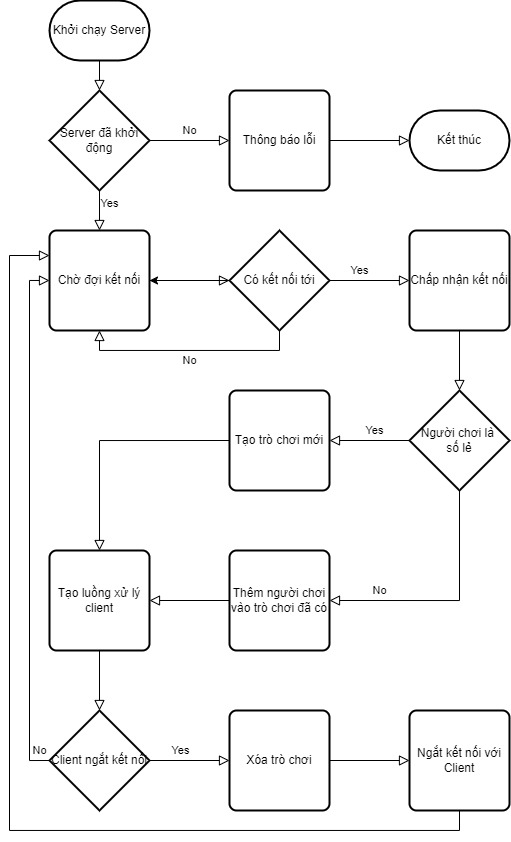
\includegraphics[width=10cm]{template_SGU/PTPMMNM_Flowchart_Server.jpg}
\end{center}
\subsubsection{Hoạt động của phần xử lý client}
\begin{center}
    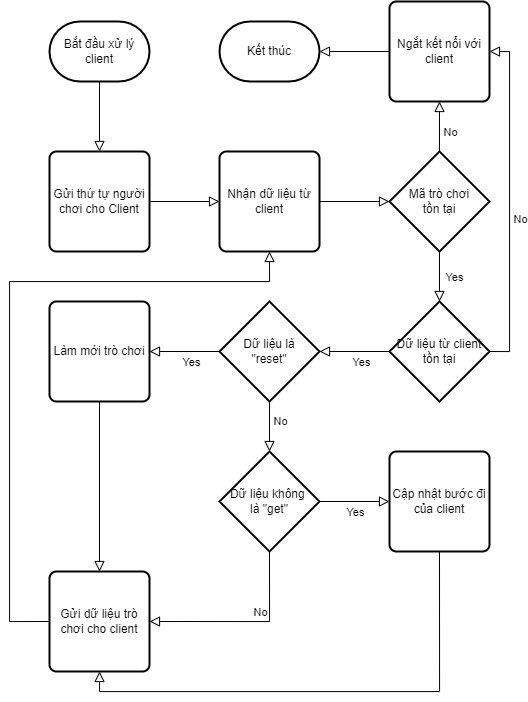
\includegraphics[width=10cm]{template_SGU/PTPMMNM_Flowchart_XulyClient.jpg}
\end{center}
\subsubsection{Hoạt động của Client}
\begin{center}
    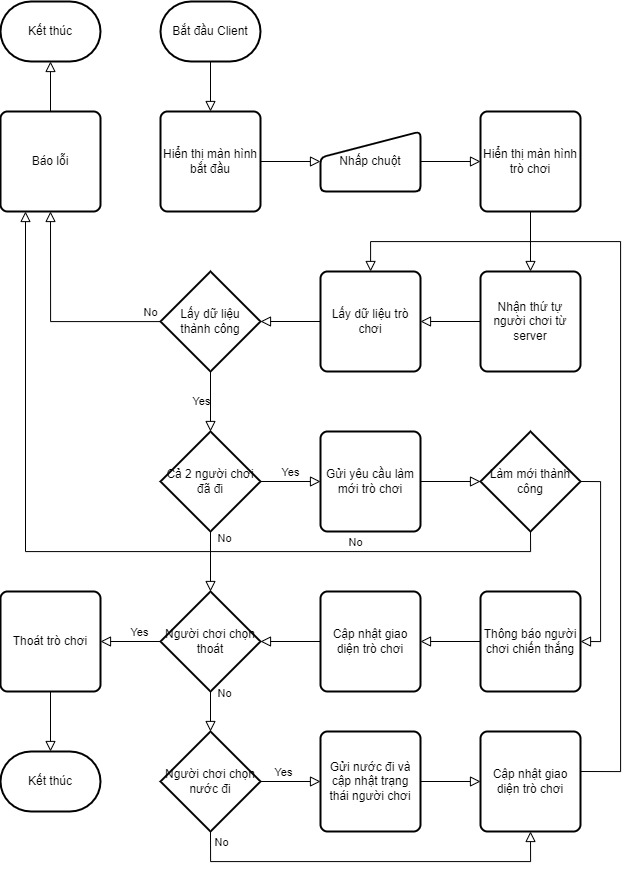
\includegraphics[width=10cm]{template_SGU/PTPMMNM_Flowchart_Client.jpg}
\end{center}

\newpage
\section{ỨNG DỤNG ĐÃ XÂY DỰNG}
\subsection{Mã nguồn}
\subsubsection{network.py}
Tệp network.py chứa mã nguồn tạo một lớp Network để quản lý việc kết nối từ client đến server trong trò chơi mạng "Kéo, Búa, Bao" (Rock, Paper, Scissors). Lớp Network cung cấp các phương thức để kết nối tới server, gửi và nhận dữ liệu một cách dễ dàng. Nó quản lý socket của client và sử dụng pickle để truyền các object phức tạp qua mạng. Các phương thức chính bao gồm:
\begin{itemize}
    \item connect: Thiết lập kết nối với server và nhận số thứ tự của người chơi.
    \item send: Gửi dữ liệu tới server và nhận lại trạng thái trò chơi từ server.
    \item getP: Trả về số thứ tự của người chơi.
Lớp này được thiết kế để tích hợp vào ứng dụng trò chơi "Kéo, Búa, Bao" (Rock, Paper, Scissors), nơi mà client cần liên tục gửi và nhận thông tin từ server để đồng bộ hóa trạng thái trò chơi.
\end{itemize}
\begin{mdframed}[hidealllines=true,backgroundcolor=magenta!10]
	\begin{lstlisting}[language=Python]
import socket
import pickle


class Network:
    def __init__(self):
        #Tao mot socket moi cho client TCP/IP.
        self.client = socket.socket(socket.AF_INET, socket.SOCK_STREAM)
        self.server = "192.168.1.8" #Dia chi IP cua server
        self.port = 5555 #Cong ma server lang nghe
        self.addr = (self.server, self.port) #chua dia chi IP va cong dung de ket noi toi server 
        self.p = self.connect() #Bien luu tru so thu tu cua nguoi choi duoc nhan tu server sau khi ket noi 

    #Phuong Thuc getP tra ve so thu tu cua nguoi choi da duoc nhan tu server 
    def getP(self):
        return self.p

    def connect(self):
        try:
            self.client.connect(self.addr) #Ket noi toi server su dung dia chi self addr 
            #Tra ve so thu tu cua nguoi choi nhan duoc tu server 
            return self.client.recv(2048).decode() #Nhan du lieu tu server so thu tu cua nguoi choi voi kich thuoc toi da 2048 byte va giai ma decode no thanh chuoi 
        #Neu xay ra loi trong qua trinh ket noi bo qua va khong lam gi trong except
        except:
            pass

    def send(self, data):
        try:
            #Gui du lieu den server sau khi ma hoa encode thanh chuoi 
            self.client.send(str.encode(data))
            #Nhan lai du lieu tu server voi kich thuoc toi da 4096 byte 2048 2 va giai tuan tu hoa deserialize no bang pickle 
            #Tra ve object da duoc giai tuan tu hoa tu server 
            return pickle.loads(self.client.recv(2048*2))
        #Neu xay ra loi trong qua trinh gui hoac nhan du lieu in ra loi
        except socket.error as e:
            print(e)
	\end{lstlisting}
\end{mdframed}
\subsubsection{server.py}
Tệp server.py chứa mã nguồn tạo ra một máy chủ (server) để quản lý trò chơi "Kéo, Búa, Bao" (Rock, Paper, Scissors) cho hai người chơi, xử lý các kết nối client và duy trì trạng thái trò chơi giữa các client. Mỗi khi một client kết nối, server sẽ xác định xem có cần tạo một trò chơi mới hay không và bắt đầu một thread mới để xử lý client đó. Các trạng thái của trò chơi được truyền qua mạng bằng cách sử dụng 'pickle'.\\
Mã nguồn này thiết lập một server TCP cho trò chơi hai người chơi, sử dụng các thư viện \_thread, pickle, socket, và một lớp Game từ module game.
 \begin{mdframed}[hidealllines=true,backgroundcolor=magenta!10]
	\begin{lstlisting}[language=Python]
import socket
from _thread import *
import pickle #Thu vien de tuan tu hoa serialize va giai tuan tu hoa deserialize cac object Python giup chung co the truyen qua mang.
from game import Game

server = "192.168.1.8"
port = 5555

s = socket.socket(socket.AF_INET, socket.SOCK_STREAM)

try:
    s.bind((server, port)) #Gan dia chi IP va cong vao socket Neu co loi bat loi va luu tru thong bao loi
except socket.error as e:
    str(e)

s.listen() #Dat socket vao che do lang nghe cac ket noi den
print("Waiting for a connection, Server Started")

connected = set()
games = {}
idCount = 0 #Bien dem so luong ket noi dung de xac dinh ID tro choi

def threaded_client(conn, p, gameId):
    global idCount
    #Gui so thu tu cua nguoi choi p den client sau khi ket noi
    conn.send(str.encode(str(p))) 

    reply = ""
    #Vong lap de lien tuc nhan du lieu tu client
    while True:
        try:
            #Nhan du lieu tu client va giai ma no thanh chuoi
            data = conn.recv(4096).decode()
            #Kiem tra xem tro choi co ton tai khong
            if gameId in games:
                #Lay doi tuong tro choi tuong ung
                game = games[gameId]

                if not data:
                    break
                else:
                    #Neu nhan duoc lenh reset thi goi ham resetWent cua tro choi
                    if data == "reset":
                        game.resetWent()
                    #Neu du lieu khong phai lenh get thi choi tro choi voi du lieu nhan duoc
                    elif data != "get":
                        game.play(p, data)
                    #Gui trang thai tro choi da duoc tuan tu hoa den client
                    conn.sendall(pickle.dumps(game))
            else:
                break
        except:
            break

    print("Lost connection")
    #Xoa tro choi khi ket noi bi mat
    try:
        del games[gameId]
        print("Closing Game", gameId)
    except:
        pass
    #Giam so luong ket noi 
    idCount -= 1
    #Dong ket noi 
    conn.close()

while True:
    conn, addr = s.accept()
    print("Connected to:", addr)
    #Tang so luong ket noi
    idCount += 1
    #Bien de xac dinh so thu tu cua nguoi choi 0 hoac 1
    p = 0
    gameId = (idCount - 1)//2
    #Neu so luong ket noi la le tao mot tro choi moi 
    if idCount % 2 == 1:
        #Tao doi tuong tro choi moi voi ID
        games[gameId] = Game(gameId)
        print("Creating a new game...")
    else:
        #Dat trang thai san sang cho tro choi
        games[gameId].ready = True
        p = 1

    #Tao mot thread moi de xu ly client
    start_new_thread(threaded_client, (conn, p, gameId))
	\end{lstlisting}
    \end{mdframed}

\subsubsection{client.py}
Tệp client.py chứa mã nguồn của một trò chơi "Kéo, Búa, Bao" (Rock, Paper, Scissors) sử dụng thư viện Pygame để tạo giao diện người dùng. Mã nguồn này kết nối với một máy chủ để chơi game trực tuyến.
\begin{mdframed}[hidealllines=true,backgroundcolor=magenta!10]
	\begin{lstlisting}[language=Python]
import pygame
from network import Network
import pickle
pygame.font.init()

width = 700
height = 700
#Xac dinh kich thuoc cua so tro choi
win = pygame.display.set_mode((width, height))
pygame.display.set_caption("Client")


class Button:
    def __init__(self, text, x, y, color):
        self.text = text
        self.x = x
        self.y = y
        self.color = color
        self.width = 150
        self.height = 100

    def draw(self, win):
        pygame.draw.rect(win, self.color, (self.x, self.y, self.width, self.height))
        font = pygame.font.SysFont("comicsans", 40)
        text = font.render(self.text, 1, (255,255,255))
        win.blit(text, (self.x + round(self.width/2) - round(text.get_width()/2), self.y + round(self.height/2) - round(text.get_height()/2)))
        
    #Kiem tra xem vi tri chuot (pos) co nam trong khu vuc nut khong.
    def click(self, pos): 
        x1 = pos[0]
        y1 = pos[1]
        if self.x <= x1 <= self.x + self.width and self.y <= y1 <= self.y + self.height:
            return True
        else:
            return False

#Ve cua so tro choi
def redrawWindow(win, game, p):
#Set background thanh mau trang
    win.fill((255, 255, 255))

    if not(game.connected()):
        #Neu game khong duoc ket noi, hien thi "Waiting for Player..."
        font = pygame.font.SysFont("comicsans", 60)
        text = font.render("Waiting for Player...", 1, (140, 120, 204), True)
        win.blit(text, (width/2 - text.get_width()/2, height/2 - text.get_height()/2))
    else:
        #Neu game duoc ket noi, hien thi cac thong bao "Your Move" va "Opponents"
        font = pygame.font.SysFont("comicsans", 60)
        text = font.render("Your Move", 1, (140, 120, 204))
        win.blit(text, (80, 200))

        text = font.render("Opponents", 1, (140, 120, 204))
        win.blit(text, (380, 200))

        #Lay thao tac cua 2 nguoi choi
        move1 = game.get_player_move(0)
        move2 = game.get_player_move(1)
        if game.bothWent():
            #Neu ca hai deu da di, hien thi nuoc di cua ho
            text1 = font.render(move1, 1, (0,0,0))
            text2 = font.render(move2, 1, (0, 0, 0))
        else:
        #Nguoc lai, neu ca hai chua move, display trang thai "Waiting..." hoac "Locked In" tuy thuoc vao tinh trang cua nguoi choi
            if game.p1Went and p == 0:
                text1 = font.render(move1, 1, (0,0,0))
            elif game.p1Went:
                text1 = font.render("Locked In", 1, (0, 0, 0))
            else:
                text1 = font.render("Waiting...", 1, (0, 0, 0))

            if game.p2Went and p == 1:
                text2 = font.render(move2, 1, (0,0,0))
            elif game.p2Went:
                text2 = font.render("Locked In", 1, (0, 0, 0))
            else:
                text2 = font.render("Waiting...", 1, (0, 0, 0))
        #Hien thi nuoc di o vi tri phu hop dua tren so thu tu (p) cua nguoi choi
        if p == 1:
            win.blit(text2, (100, 350))
            win.blit(text1, (400, 350))
        else:
            win.blit(text1, (100, 350))
            win.blit(text2, (400, 350))
        #Ve cac button len cua so
        for btn in btns:
            btn.draw(win)
    #Cap nhat man  hinh de hien thi cac thay doi
    pygame.display.update()

#Tao 3 button cho cac lua chon "Rock", "Scissors" va "Paper"
btns = [Button("Rock", 50, 500, (146, 146, 214)), Button("Scissors", 250, 500, (146, 146, 214)), Button("Paper", 450, 500, (146, 146, 214))]

def main():
    run = True #Bien dieu khien vong lap chinh cua tro choi
    clock = pygame.time.Clock() #Tao doi tuong clock kiem soat toc do khung hinh cua Pygame
    n = Network()
    player = int(n.getP()) #Lay so thu tu cua nguoi choi tu server
    print("You are player", player)

    while run:
        clock.tick(60)
        try:
            game = n.send("get") #Gui yeu cau 'get' toi server de   lay thong tin ve trang thai tro choi
        except:
            run = False
            print("Couldn't get game")
            break

        if game.bothWent():
            redrawWindow(win, game, player)
            pygame.time.delay(500)
            try:
                game = n.send("reset") #Gui yeu cau cau 'reset' toi server de dat lai trang thai tro choi
            except:
                run = False
                print("Couldn't get game")
                break
            #Hien thi ket qua tro choi
            font = pygame.font.SysFont("comicsans", 80)
            if (game.winner() == 1 and player == 1) or (game.winner() == 0 and player == 0):
                text = font.render("You Won!", 1, (0,255,0))
            elif game.winner() == -1:
                text = font.render("Tie Game!", 1, (255,255,0))
            else:
                text = font.render("You Lost...", 1, (255, 0, 0))

            win.blit(text, (width/2 - text.get_width()/2, height/2 - text.get_height()/2))
            pygame.display.update()
            pygame.time.delay(2000)
        #Lap qua tat ca su kien da xay ra
        for event in pygame.event.get():
            if event.type == pygame.QUIT:
                run = False
                pygame.quit()
            
            if event.type == pygame.MOUSEBUTTONDOWN:
                pos = pygame.mouse.get_pos()    #Lay vi tri con tro chuot
                for btn in btns:
                    #Kiem tra vi tri nhap chuot co nam trong pham vi cua nut hay khong và tro choi da san sang chua
                    if btn.click(pos) and game.connected():
                        if player == 0:
                            if not game.p1Went:
                                n.send(btn.text)
                        else:
                            if not game.p2Went:
                                n.send(btn.text)

        redrawWindow(win, game, player)
#Hien thi man hinh menu cho nguoi choi nhap chuot de bat dau tro choi. Khi nguoi choi nhap chuot, ham 'main' duoc goi de bat dat tro choi
def menu_screen():
    run = True
    clock = pygame.time.Clock()

    while run:
        clock.tick(60)
        win.fill((255, 255, 255))
        font = pygame.font.SysFont("comicsans", 60)
        text = font.render("Click to Play!", 1, (140, 120, 204))
        win.blit(text, (200,250))
        pygame.display.update()

        for event in pygame.event.get():
            if event.type == pygame.QUIT:
                pygame.quit()
                run = False
            if event.type == pygame.MOUSEBUTTONDOWN:
                run = False

    main()
#Vong lap de hien thi man hinh menu lien tuc
while True:
    menu_screen()

	\end{lstlisting}
	\end{mdframed}
\subsubsection{game.py}
Tệp 'game.py' chứa định nghĩa của lơp 'Game'. Lớp Game này quản lý trạng thái và logic của trò chơi "Kéo, Búa, Bao" giữa hai người chơi. Nó theo dõi các nước đi của người chơi, xác định người thắng cuộc, và quản lý các trạng thái khác của trò chơi như kết nối và sẵn sàng.
\begin{mdframed}[hidealllines=true,backgroundcolor=magenta!10]
	\begin{lstlisting}[language=Python]
class Game:
    def __init__(self, id):
        self.p1Went = False
        self.p2Went = False
        self.ready = False
        self.id = id
        self.moves = [None, None]
        self.wins = [0,0]
        self.ties = 0
    #return nuoc di cua nguoi choi duoc chi dinh
    def get_player_move(self, p): 
        """
        :param p: [0,1]
        :return: Move
        """
        return self.moves[p]
    #Cap nhat nuoc di cua nguoi choi (0 hoac 1) voi gia tri 'move'
    def play(self, player, move):
        self.moves[player] = move
        if player == 0:
            self.p1Went = True
        else:
            self.p2Went = True
    #Tra ve gia tri cua 'self.ready' de kiem tra xem tro choi da san sang chua
    def connected(self):
        return self.ready
    #Kiem tra xem ca hai nguoi choi da thuc hien nuoc di cua ho chua
    def bothWent(self):
        return self.p1Went and self.p2Went
    #Ham xac dinh nguoi thang
    def winner(self):
        #Nuoc di duoc chuyen thanh chu hoa va lay ky tu dau tien, de dam bao rang no la 'R;, 'P' hoac 'S'
        p1 = self.moves[0].upper()[0]
        p2 = self.moves[1].upper()[0]

        winner = -1
        if p1 == "R" and p2 == "S":
            winner = 0
        elif p1 == "S" and p2 == "R":
            winner = 1
        elif p1 == "P" and p2 == "R":
            winner = 0
        elif p1 == "R" and p2 == "P":
            winner = 1
        elif p1 == "S" and p2 == "P":
            winner = 0
        elif p1 == "P" and p2 == "S":
            winner = 1
        # Tra ve '0' neu nguoi choi 1 thang, '1' neu nguoi choi 2 thang va '-1' neu hoa
        return winner
    #Dat lai 2 bien co thanh 'False' de chuan bi cho luot choi tiep theo
    def resetWent(self):
        self.p1Went = False
        self.p2Went = False
	\end{lstlisting}
	\end{mdframed}
\subsection{Hình ảnh giao diện}
\subsubsection{Giao diện chờ kết nối vào game}
Sau khi chạy lệnh 'python client.py' trên command line, giao diện chờ kết nối vào game với nội dung "Click to Play!" sẽ được hiển thị để chờ thao tác click từ người dùng/
\begin{center}
    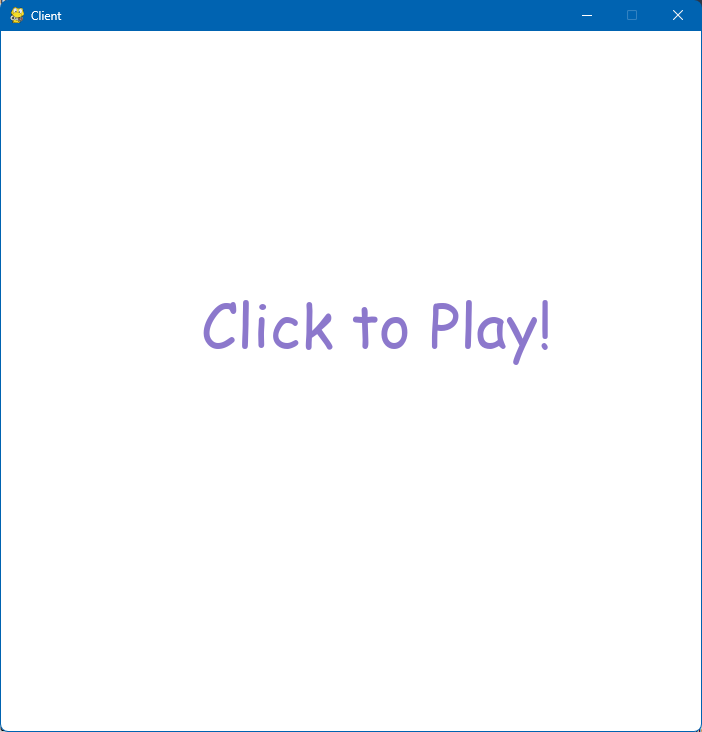
\includegraphics[width=10cm]{template_SGU/UI_WatingConnection.png}
\end{center}
\subsubsection{Giao diện chờ thao tác kết nối vào game từ người chơi còn lại}
Sau khi người chơi click vào màn hình giao diện chờ kết nối, màn hình sẽ thay đổi thành "Waiting for Player" để chờ kết nối từ người chơi còn lại.
\begin{center}
    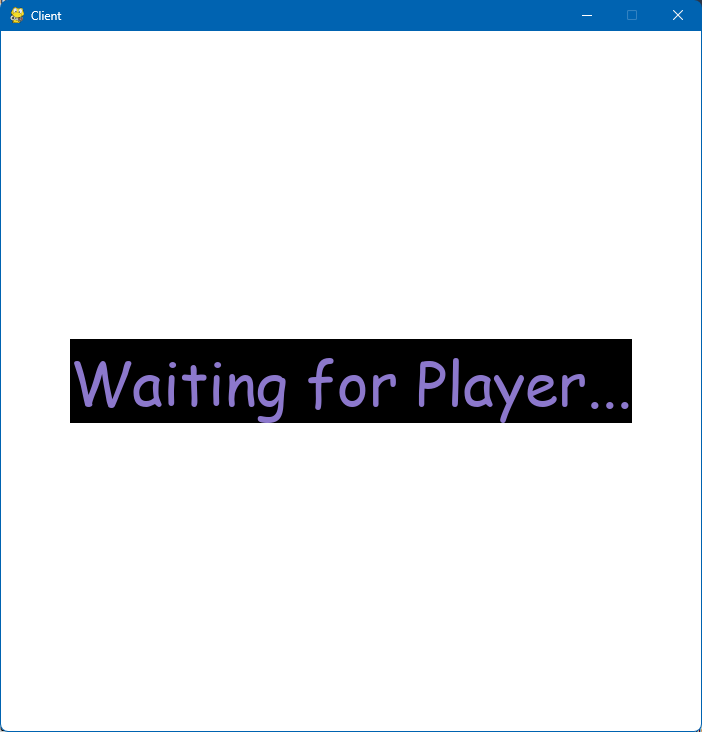
\includegraphics[width=10cm]{template_SGU/UI_WaitingPlayer.png}
\end{center}
\subsubsection{Giao diện game chính}
Sau khi cả hai người chơi đều click vào giao diện chờ kết nối, giao diện game chính được hiển thì, giao diện chia màn hình ra thành 2 phần, phần bên trái thể hiện nước đi của người chơi hiện tại với nội dung "Your Move", phần bên phải sẽ hiển thị nước đi của đối phương với nội dung "Opponents". Bên dưới hiển thị 3 button tương ứng với lựa chọn nước đi của người chơi.
\begin{center}
    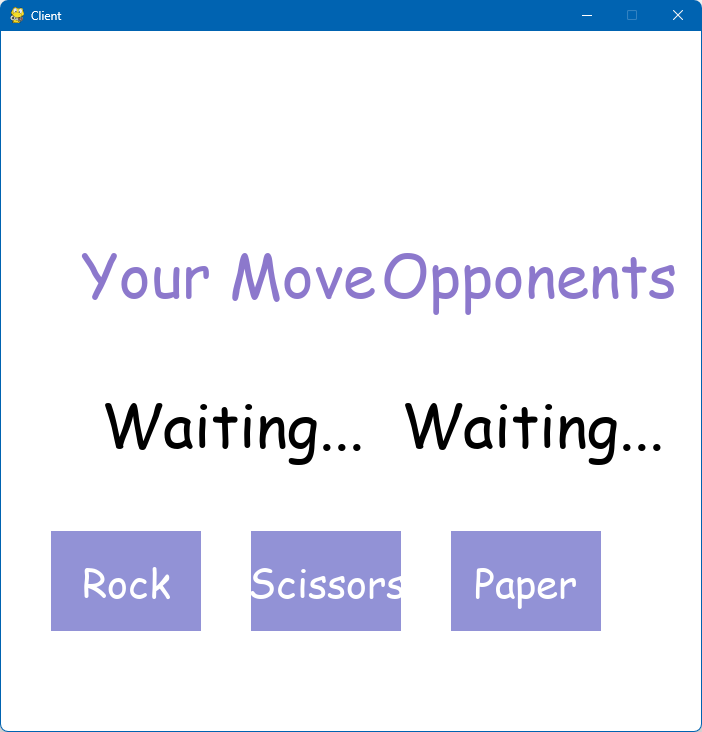
\includegraphics[width=10cm]{template_SGU/UI_Main.png}
\end{center}
\subsubsection{Giao diện chờ lượt chơi từ người chơi còn lại}
Người chơi sau khi chọn 1 trong 3 nước đi, màn hình sẽ cập nhật nước đi cho người chơi hiện tại và chờ nước đi từ đối thủ của họ.
\begin{center}
    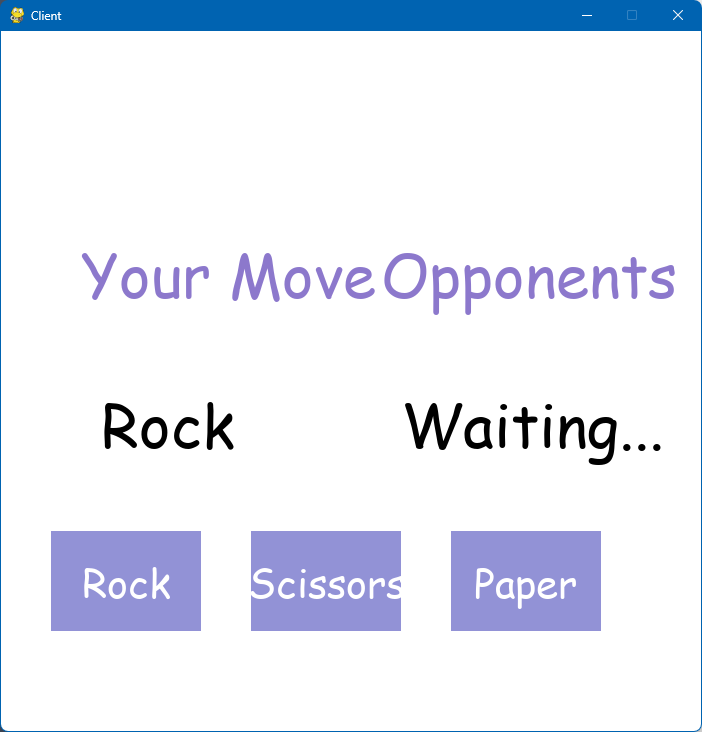
\includegraphics[width=10cm]{template_SGU/UI_WaitingOpponentMove.png}
\end{center}
Khi đối thủ đã chọn nước đi, bên Opponents sẽ cập nhật thành "Locked In" và chờ nước đi từ người chơi hiện tại.
\begin{center}
    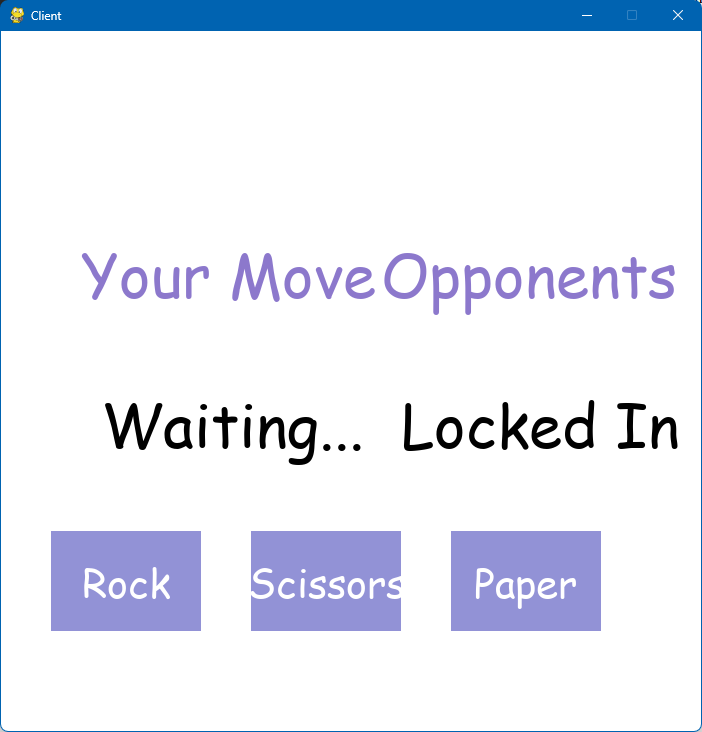
\includegraphics[width=10cm]{template_SGU/UI_WaitingMovement.png}
\end{center}

\subsubsection{Giao diện thắng}
Giao diện hiển thị kết quả người chơi đã thắng với nội dung "You Won!"
\begin{center}
    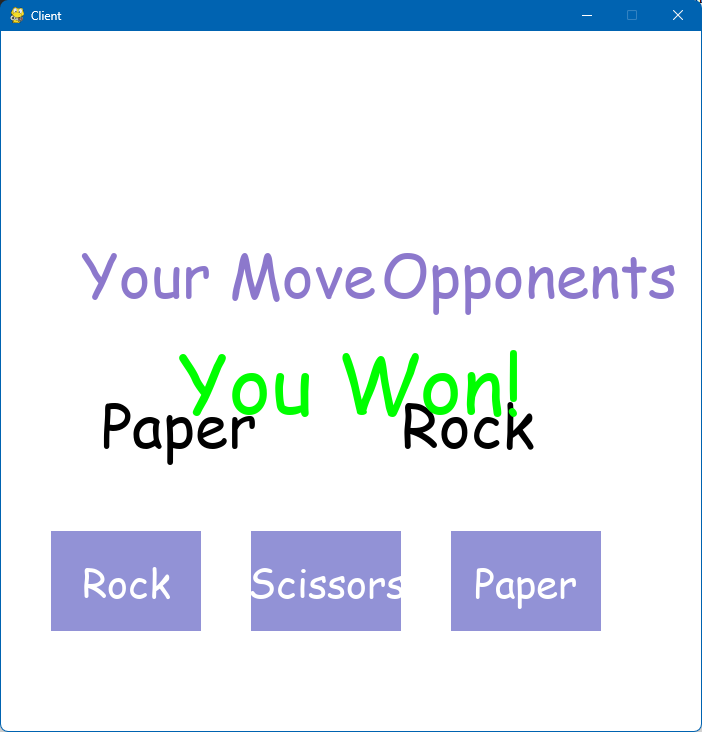
\includegraphics[width=10cm]{template_SGU/UI_Win.png}
\end{center}
\subsubsection{Giao diện hòa}
Giao diện hiển thị kết quả hòa với nội dung "Tie Game!"
\begin{center}
    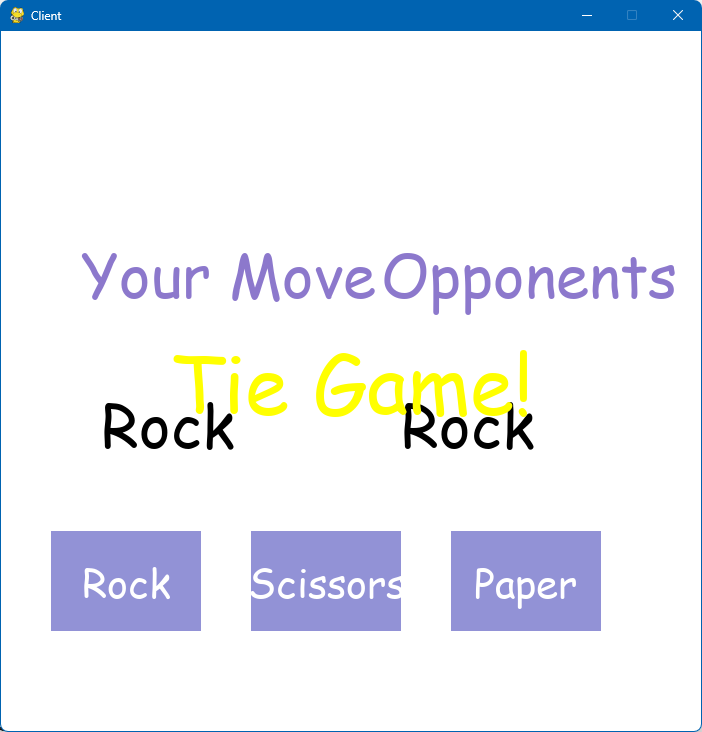
\includegraphics[width=10cm]{template_SGU/UI_Tie.png}
\end{center}
\subsubsection{Giao diện thua}
Giao diện hiển thị kết quả người chơi đã thua với nội dung "You Lost..."
\begin{center}
    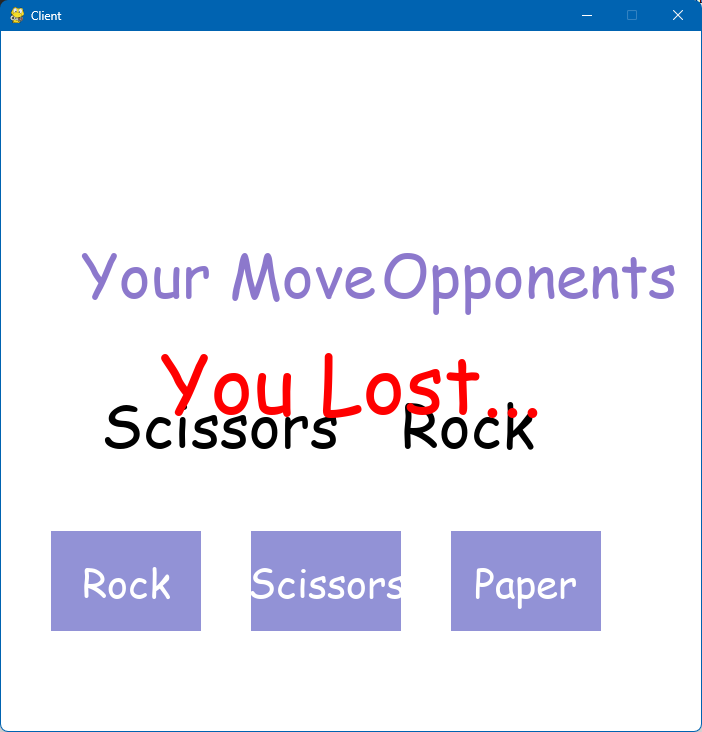
\includegraphics[width=10cm]{template_SGU/UI_Lost.png}
\end{center}
\newpage
\section{CÁCH THỨC CÀI ĐẶT ỨNG DỤNG}
\subsection{Cài đặt}
Đầu tiền, ta cần phải cài đặt thư viện PyGame bằng lệnh:\\
\indent {\tt pip install pygame}\\
Sau đó, ta sẽ clone dự án từ link github: https://github.com/giaphat-nham/Rock-Paper-and-Scissors-Multiplayer-Game, bằng lệnh sau:\\
\indent {\tt git clone <Đường dẫn đến repository>}\\
Vậy là ta đã xong phần cài đặt.
\subsection{Cấu hình}
Tiếp theo, ta cần phải cấu hình mã nguồn cho phù hợp với thiết bị của chúng ta. Cụ thể hơn là cấu hình địa chỉ IP của server. Ta mở file {\tt server.py} sau đó ghi địa chỉ IP của máy chủ mà ta chọn làm host tại dòng {\tt server = ...} Ta cũng sẽ ghi địa chỉ IP của máy chủ vào file {\tt network.py} tại dòng {\tt self.server = ...}\\
Vậy là bây giờ chúng ta có thể tiến hành chạy trò chơi.
\subsection{Chạy trò chơi}
Để chạy trò chơi, đầu tiên tại máy làm máy chủ, ta sẽ sử dụng lệnh:\\
{\tt python server.py}\\
Lúc này máy chủ đã được khởi động thành công. Với mỗi người chơi muốn tham gia vào trò chơi, họ sẽ sử dụng lệnh:\\
{\tt python client.py}\\
Sau khi gõ lệnh, cửa sổ trò chơi sẽ hiển thị trên màn hình của người chơi, và hai người chơi có thể chơi với nhau.
\newpage
\section{PHẦN CÔNG CÔNG VIỆC GIỮA CÁC THÀNH VIÊN}

\begin{table}[h]
    \centering
    \begin{tabular}{|p{2cm}|p{8cm}|}
        \hline
        \textbf{Tên thành viên} &\textbf{Công việc} \\
        \hline
         Lê Quỳnh Thiên Hương& Viết báo cáo phần Cơ sở lý thuyết Pygame; Mã nguồn client.py, game.py; Mô tả hình ảnh giao diện \\
         \hline
         Bùi Thị Yến Nhi& Viết báo cáo phần Cơ sở lý thuyêt Socket trong Python; Mã nguồn server.py và network.py \\
         \hline
         Nhâm Gia Phát&Xây dựng code ứng dụng, Viết báo cáo phần Thiết kế ứng dụng\\
         \hline
    \end{tabular}
    \caption{Bảng phân công công việc}
    \label{tab:my_label}
\end{table}

\newpage
\begin{thebibliography}{80}

\bibitem{Youtube}
freeCodeCamp.org(27/03/2019).
``\textbf{link: https://t.ly/A4go-}'',
\textit{Python Online Multiplayer Game Development Tutorial}, lần truy cập cuối: 05/05/2024.

\bibitem{Geeksforgeeks}
Geeksforgeeks(12/03/2024).
``\textbf{link: https://www.geeksforgeeks.org/pygame-tutorial/}'',
\textit{PyGame Tutorial}, lần truy cập cuối: 05/05/2024.

\bibitem{w3schools}
W3Schools.
``\textbf{link: https://www.w3schools.com/python}'',
\textit{Python Tutorial}, lần truy cập cuối: 05/05/2024.

\end{thebibliography}
\end{document}

